\documentclass[10pt]{article}

\input{/Users/gabesekeres/Dropbox/LaTeX_Docs/pset_preamble.tex}

\course{ECON 6100}
\pset{4}
\begin{document}
\maketitle

\begin{enumerate}
	\item Building a Ricardian trade model between England and Spain from scratch. 
	\begin{enumerate}
		\item To construct the global production possibilities frontier, we will assume that each country has a comparative advantage in a different good. Following tradition, assume that England has a comparative advantage in mutton and Spain has a comparative advantage in wine. We have the two individual production possibility sets, for a certain level of production, in Figure~\ref{fig:indiv_ppf}. 
		\begin{figure}[H]
			\centering
			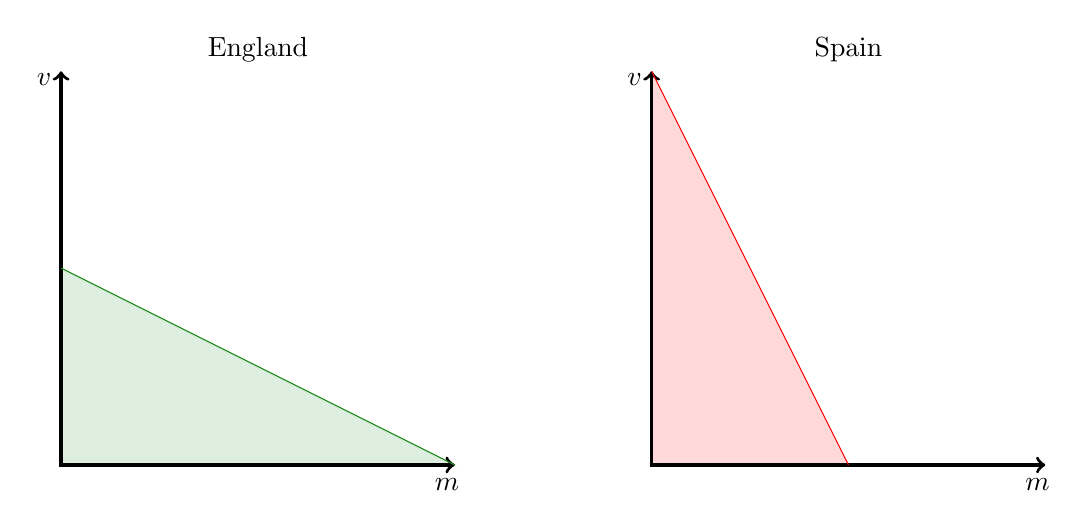
\begin{tikzpicture}[scale=0.5]
				\filldraw[ForestGreen!15] (0,5)--(10,0)--(0,0)--(0,5);
				\filldraw[red!15] (15,10)--(20,0)--(15,0)--(15,10);
				
				\draw[very thick,<->] (10,0)--(0,0)--(0,10);
				\draw[very thick,<->] (25,0)--(15,0)--(15,10);
				\node[above] at (5,10) {England};
				\node[above] at (20,10) {Spain};
				\node[left] at (0,9.8) {$v$};
				\node[left] at (15,9.8) {$v$};
				\node[below] at (9.8,-0.1) {$m$};
				\node[below] at (24.8,-0.1) {$m$};
				\draw[ForestGreen] (0,5)--(10,0);
				\draw[red] (15,10)--(20,0);
			\end{tikzpicture}
			\caption{Production Posibility Sets for England and Spain}
			\label{fig:indiv_ppf}
		\end{figure}
		Summing them up, we can get the global production possibilities frontier, in Figure~\ref{fig:global_ppf}.
		\begin{figure}[H]
			\centering
			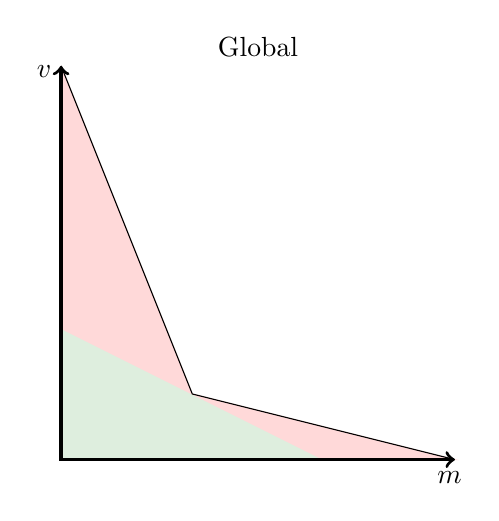
\begin{tikzpicture}[scale=0.3333333]
				\filldraw[ForestGreen!15] (0,5)--(10,0)--(0,0)--(0,5);
				\filldraw[red!15] (0,15)--(5,2.5)--(15,0)--(10,0)--(5,2.5)--(0,5)--(0,15);
				\draw[<->,very thick] (15,0)--(0,0)--(0,15);
				\node[left] at (0,14.8) {$v$};
				\node[below] at (14.8,-0.1) {$m$};
				\draw (0,15)--(5,2.5)--(15,0);
				\node[above] at (7.5,15) {Global};
			\end{tikzpicture}
			\caption{Global Production Possibility Set}
			\label{fig:global_ppf}
		\end{figure}
		We define England's labor stock as $L_E$ and Spain's labor stock as $L_S$, and each country has a (different) labor requirement vector $a^0_E$, $a^0_S$ respectively. England and Spain can also trade goods with each other, at a certain ratio determined by $p_v$ and $p_m$, the prices. At a certain point $x$ on the global production possibility frontier, the countries are both using the entirety of their labor stock. Each country will be producing the good that they're better at more than the good that they're worse at.
		\item This model says that a market equilibrium is a trade equilibrium between the two countries, where they each consume a certain amount in ratio to the price vector. Moreover, if the two labor requirement vectors are different, then there exist prices at which each country produces only the good that they have a comparative advantage in and they trade.
		\item Observe that if trade is positive (\ie if each country produces a good cheaper than the other), then that means that each country has a comparative advantage in the good that they produce. Moreover, for any reasonable utility functions, if trade is positive then each country will produce only the good that they are better at producing.
		\item An efficient producer will produce a point on their own production possibility frontier. In equilibrium, both producers will of course be efficient here (as long as the goods are actually good).
		\item England has a production matrix $A_E \in \reals^{2 \times 2}$, where $a^0_E$ is the labor requirement vector. Spain has a production matrix $A_S \in \reals^{2 \times 2}$, where $a^0_S$ is the labor requirement vector. Now, England can produce $(I-A_E)^{-1}y$ of its own goods, and Spain can produce $(I-A_S)^{-1}y$ of its own goods. We no longer can use an easy story of comparative advantage, but the countries may still be incentivized to trade with each other. The pattern of trade could be the reverse, if wine is an input for mutton and vice versa. In that case, Spain would be very good at producing inputs for mutton and thus mutton, and vice versa for England, so they would trade in the other direction.
		\item If we add shipping costs which reduce the amount of inputs that go from one direction to the other, it is no longer so clear that the countries will trade everything and produce only one good. Instead, trade will need to be worth more than both the comparative price of production and the loss from shipping. If that does not hold, then the countries would rather use an autarkic regime.
		\item Equilibrium is dual to productive efficiency in the sense that production is efficient if and only if there is full trade in equilibrium. We could formulate the maximization problem as `maximize (utility from) consumption subject to trade and labor being fulfilled'. Then the dual problem is `minimize total costs to attain a certain utility from consumption'. As in producer theory, the two problems are dual and strong duality holds, meaning that the equilibrium will be the same no matter the formulation.
	\end{enumerate}
\end{enumerate}
































\end{document}